\chapter{Results}
\label{ch:results}
\epigraph{\itshape``What could I say to you that would be of value, except that perhaps you seek too much, that as a result of your seeking you cannot find. "}{--- \textup{Hermann Hesse}}
\mediumlinespacing

\section{Introduction}
\hspace{10pt} This chapter serves as a summary of results arising from measurements defined by previously introduced strategy. Majority of the following sections are going to be dedicated to measurements through the usage of data collected by the CMS experiment during the 2017 and 2018 eras of data taking. A discussion of benefits rising due to the inclusion of a new analysis category, formed around the VBF triggers, is also presented. Final result from the VBF analysis from the perspective of the full Run 2 era is obtained through a combination with, previously published, study detailing the analysis of 2016 data~\cite{paper:HIG_17_023}.
\newpage
\section{Fit results}

\hspace{10pt} The signal extraction procedure introduced in previous sections is applied to all regions simultaneously. The following sections summarise the final results, expressed in terms of the 95~\% CL upper limit on Br(H$\rightarrow$~inv) for both analysis categories which are ultimately combined. In order to formulate a preliminary look at the combined Run 2 result (or the "legacy"), a combination is performed with the studies targeting the 2016 data without re-analysing the data (being explained in great detail in Refs. [R,R]). Correlation of most important nuisance parameters such as the ones related to lepton efficiencies have been left uncorrelated between the three years. Uncertainties assigned to the jet energy scale and resolution are also following the uncorrelated path. On the other hand, a correlation between theory uncertainty has been established between 2017 and 2018 (although they differ between MTR and VTR categories). The addition of the photon region has been performed for the MTR category for the 2017 and 2018 eras of data taking.

\hspace{10pt} Starting with the main analysis category, Figures~[R]-[R] show postfit distributions for the main CRs and the SR. Table~[R] presents the final yields in the SR for the MTR category. No excess is present at the moment TBA discussion of the results.

\hspace{10pt} The resulting postfit distributions associated to the VTR category are shown in Figures~[R]-[R]. The corresponding yields of data and simulated SM processes are given in Tables~[R]-[R].

\begin{sidewaystable}[]
    \centering
    \footnotesize
\begin{tabular}{l|c|c|c|c|c|c|c|c|c}
Process & 200-400 & 400-600 & 600-900 & 900-1200 & 1200-1500 & 1500-2000 & 2000-2750 & 2750-3500 & $>$3500  \\
\hline
\hline
$\cPZ(\nu\nu)+\textrm{jets}$ (strong)  & $13301.1\pm421.8$ & $7766.5\pm262.8$ & $5505.9\pm180.0$ & $2256.7\pm88.8$ & $1010.9\pm41.8$ & $649.2\pm32.3$ & $256.9\pm14.5$ & $53.1\pm5.9$ & $15.4\pm2.6$\\
$\cPZ(\nu\nu)+\textrm{jets}$ (VBF)  & $228.0\pm9.1$ & $273.1\pm11.8$ & $297.9\pm11.7$ & $194.7\pm8.8$ & $130.7\pm6.9$ & $125.4\pm7.0$ & $87.5\pm6.4$ & $25.7\pm3.0$ & $15.2\pm2.7$\\
$\PW(\ell\nu)+\textrm{jets}$ (strong)  & $6343.3\pm271.5$ & $4005.3\pm183.3$ & $2933.9\pm132.3$ & $1310.1\pm64.7$ & $599.0\pm33.4$ & $388.9\pm24.4$ & $160.9\pm13.4$ & $31.3\pm5.2$ & $8.1\pm2.1$\\
$\PW(\ell\nu)+\textrm{jets}$ (VBF)  & $131.4\pm15.3$ & $152.1\pm16.0$ & $162.4\pm16.7$ & $106.7\pm12.2$ & $84.0\pm9.4$ & $76.5\pm7.7$ & $47.3\pm4.9$ & $15.9\pm2.6$ & $9.1\pm1.7$\\
$\ttbar$ + single-top  & $210.8\pm21.2$ & $144.8\pm14.0$ & $164.3\pm15.8$ & $49.2\pm7.4$ & $19.7\pm4.8$ & $16.7\pm1.6$ & $8.3\pm2.1$ & $1.2\pm0.3$ & $0.9\pm0.1$\\
Diboson  & $225.5\pm21.5$ & $148.3\pm14.1$ & $115.4\pm11.0$ & $44.3\pm4.4$ & $18.7\pm1.8$ & $9.2\pm0.9$ & $3.1\pm0.3$ & $0.8\pm0.1$ & $0.3\pm0.0$\\
$\cPZ/\gamma^{*}(\ell^{+}\ell^{-})+\mathrm{jets}$  & $79.5\pm4.2$ & $56.9\pm2.9$ & $45.3\pm2.1$ & $20.3\pm0.8$ & $10.9\pm0.4$ & $7.1\pm0.4$ & $1.7\pm0.1$ & $0.2\pm0.0$ & $0.2\pm0.0$\\
Multijet  & $19.0\pm6.7$ & $20.7\pm7.2$ & $27.9\pm9.8$ & $15.2\pm5.3$ & $8.9\pm3.1$ & $9.3\pm3.3$ & $6.4\pm2.2$ & $3.4\pm1.2$ & $3.4\pm1.2$\\
\hline
$\mathrm{gg}\PH(\rightarrow \mathrm{inv.})$  & $288.0$ & $212.8$ & $169.4$ & $82.2$ & $44.2$ & $46.5$ & $15.8$ & $5.0$ & $0.0$\\
$\mathrm{qq}\PH(\rightarrow \mathrm{inv.})$  & $33.6$ & $72.4$ & $137.2$ & $129.1$ & $105.0$ & $112.6$ & $86.1$ & $28.7$ & $20.2$\\
\hline
Observed & 0 & 0 & 0 & 0 & 0 & 0 & 0 & 0 & 0\\
\hline
\end{tabular}
    \caption{Caption - 2017}
    \label{tab:my_label}
\end{sidewaystable}


\begin{sidewaystable}[]
    \centering
    \footnotesize
\begin{tabular}{l|c|c|c|c|c|c|c|c|c}
Process & 200-400 & 400-600 & 600-900 & 900-1200 & 1200-1500 & 1500-2000 & 2000-2750 & 2750-3500 & $>$3500  \\
\hline
\hline
$\cPZ(\nu\nu)+\textrm{jets}$ (strong)  & $13301.1\pm421.8$ & $7766.5\pm262.8$ & $5505.9\pm180.0$ & $2256.7\pm88.8$ & $1010.9\pm41.8$ & $649.2\pm32.3$ & $256.9\pm14.5$ & $53.1\pm5.9$ & $15.4\pm2.6$\\
$\cPZ(\nu\nu)+\textrm{jets}$ (VBF)  & $228.0\pm9.1$ & $273.1\pm11.8$ & $297.9\pm11.7$ & $194.7\pm8.8$ & $130.7\pm6.9$ & $125.4\pm7.0$ & $87.5\pm6.4$ & $25.7\pm3.0$ & $15.2\pm2.7$\\
$\PW(\ell\nu)+\textrm{jets}$ (strong)  & $6343.3\pm271.5$ & $4005.3\pm183.3$ & $2933.9\pm132.3$ & $1310.1\pm64.7$ & $599.0\pm33.4$ & $388.9\pm24.4$ & $160.9\pm13.4$ & $31.3\pm5.2$ & $8.1\pm2.1$\\
$\PW(\ell\nu)+\textrm{jets}$ (VBF)  & $131.4\pm15.3$ & $152.1\pm16.0$ & $162.4\pm16.7$ & $106.7\pm12.2$ & $84.0\pm9.4$ & $76.5\pm7.7$ & $47.3\pm4.9$ & $15.9\pm2.6$ & $9.1\pm1.7$\\
$\ttbar$ + single-top  & $210.8\pm21.2$ & $144.8\pm14.0$ & $164.3\pm15.8$ & $49.2\pm7.4$ & $19.7\pm4.8$ & $16.7\pm1.6$ & $8.3\pm2.1$ & $1.2\pm0.3$ & $0.9\pm0.1$\\
Diboson  & $225.5\pm21.5$ & $148.3\pm14.1$ & $115.4\pm11.0$ & $44.3\pm4.4$ & $18.7\pm1.8$ & $9.2\pm0.9$ & $3.1\pm0.3$ & $0.8\pm0.1$ & $0.3\pm0.0$\\
$\cPZ/\gamma^{*}(\ell^{+}\ell^{-})+\mathrm{jets}$  & $79.5\pm4.2$ & $56.9\pm2.9$ & $45.3\pm2.1$ & $20.3\pm0.8$ & $10.9\pm0.4$ & $7.1\pm0.4$ & $1.7\pm0.1$ & $0.2\pm0.0$ & $0.2\pm0.0$\\
Multijet  & $19.0\pm6.7$ & $20.7\pm7.2$ & $27.9\pm9.8$ & $15.2\pm5.3$ & $8.9\pm3.1$ & $9.3\pm3.3$ & $6.4\pm2.2$ & $3.4\pm1.2$ & $3.4\pm1.2$\\
\hline
$\mathrm{gg}\PH(\rightarrow \mathrm{inv.})$  & $288.0$ & $212.8$ & $169.4$ & $82.2$ & $44.2$ & $46.5$ & $15.8$ & $5.0$ & $0.0$\\
$\mathrm{qq}\PH(\rightarrow \mathrm{inv.})$  & $33.6$ & $72.4$ & $137.2$ & $129.1$ & $105.0$ & $112.6$ & $86.1$ & $28.7$ & $20.2$\\
\hline
Observed & 0 & 0 & 0 & 0 & 0 & 0 & 0 & 0 & 0\\
\hline
\end{tabular}
    \caption{2018}
    \label{tab:my_label}
\end{sidewaystable}



\newpage
\section{Summary}
\hspace{10pt} The presented study covered the search for the invisible decays of the Higgs boson, where the production mode in question is VBF, The study was performed using the 101.3~$fb^{-1}$ of data collected by the CMS experiment. Exploration of additional phase space found in lower $E_{T,miss}$ range was enabled through the introduction of a new analysis category based on new trigger algorithms tailored to look for the VBF topology. No deviations from the SM have been observed. The result is interpreted as the observed (expected) 95\% CL upper limit on the branching ratio of the Higgs boson decaying invisibly and it stands at: Br(H$\rightarrow$inv) = XX (XX). A combination with previous measurements targeting the VBF topology during the Run 2 phase is presented, bringing the total integrated luminosity to 137.2~$fb^{-1}$. The observed (expected) value of the Br(H$\rightarrow$inv) for the entire Run 2 phase is found to be XX (XX)\footnote{Under the assumption of the SM production cross section.}. Figure~\ref{fig:combined_limit} summarised the results of the individual measurements and the subsequent combination of categories.

\begin{figure}[htbp]
  \centering
    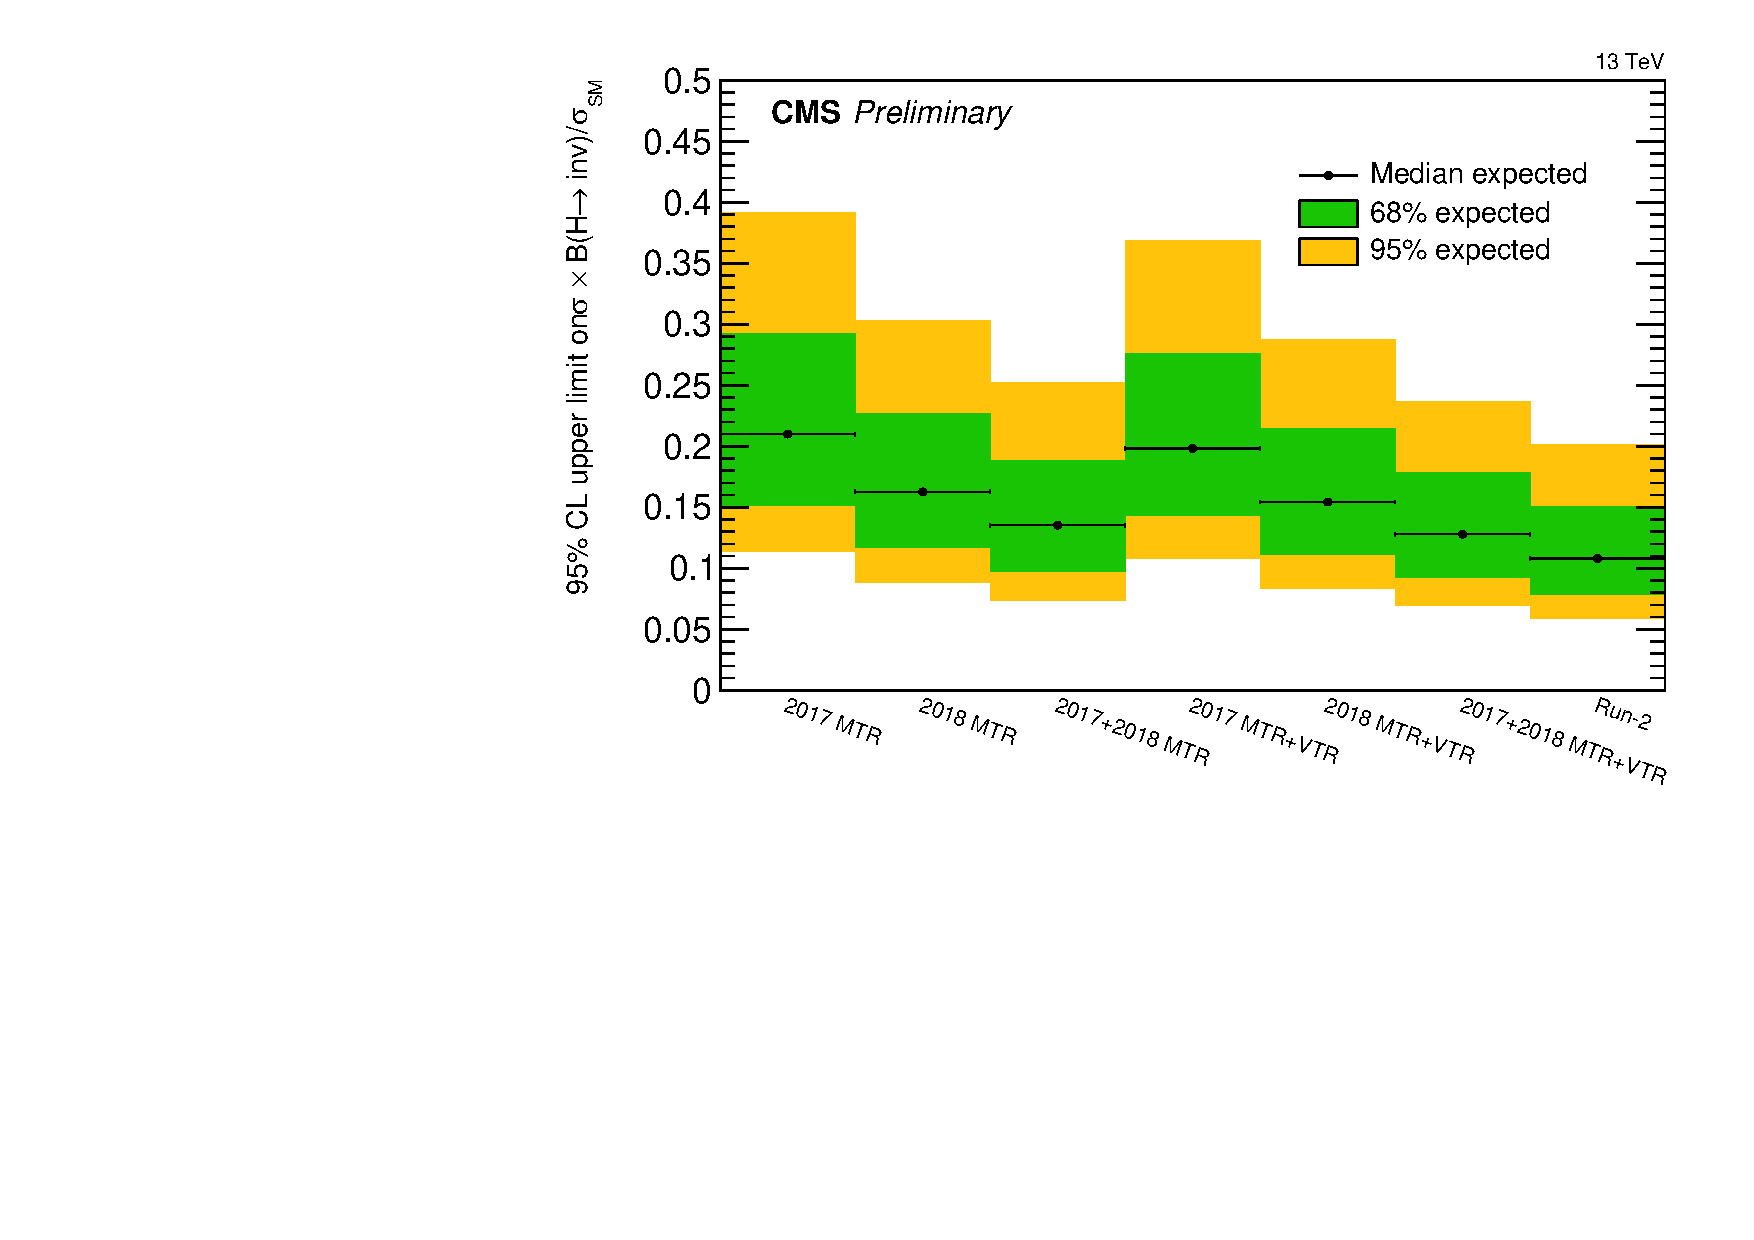
\includegraphics[width= 0.95\textwidth]{Results/limit.pdf}
  \caption{Combined limit.}
  \label{fig:combined_limit}
\end{figure}